\chapter{Grundbegriffe}

\section{Threads}

\begin{description}
\item[Prozess] Sequentieller Rechenvorgang
\item[sequentiell] Alle Rechenschritte laufen nacheinander in einer vorgegebenen Reihenfolge ab.
\item[Thread] "`leichte"' Variante eines Prozesses
\end{description}

Allgemeine Tendenz:
\begin{enumerate}
\item Systemkern möglichst "`schlank"' halten
\item Systemkern möglichst selten betreten
\end{enumerate}

Unterschied zu Prozess:
\begin{itemize}
\item Kein eigener Speicherbereich
\item Üblicherweise nicht vom Systemkern verwaltet ("`leight-weight process"'), vom Systemkern verwaltet
\end{itemize}

Vorteile:
\begin{itemize}
\item Wechsel zwischen Threads weniger aufwändig als Wechsel zwischen Prozessen
\item Threads benötigen weniger Speicher
\item Man kann viel mehr Threads ($\approx$ 10.000) als Prozesse ($\approx$ 100) laufen lassen.
\end{itemize}

Nachteil:\\
Anwendungsprogrammierer muss sich um Verwaltung der Threads kümmern. Viele Programmiersprachen bieten heutzutage Programmbibliotheken für Threads an (Beispiel: \emph{PThread} in C). Wir verwenden in dieser Veranstaltung \emph{Java} als Programmiersprache.

\begin{description}
\item[parallel] Mehrere Threads laufen gleichzeitig auf verschiedenen Rechnerkernen.
\item[verschränkt (engl. interleaved)] Threads laufen abwechselnd je ein Stück weit.
\item[nebeneinander laufend (auch: nebenläufig, engl. concurrent)] Mehrere Threads laufen parallel oder miteinander verschränkt.
\end{description}

Auch Mischformen sind möglich.
\subsubsection*{Unterschied:}
\begin{description}
\item[Rechenzeit (engl. cpu time)] Zeit, die der Prozessor mit Rechnen zubringt.
\item[Bearbeitungszeit (engl. wall clock time)] Umfasst auch Wartezeiten.
\end{description}

\subsubsection*{Amdahlsches Gesetz (Gene Amdahl, 1967):}
Wenn eine Aufgabe die Bearbeitungszeit $ a $ benötigt und der Anteil $ 0 \leq p \leq 1 $ davon parallelisierbar ist, dann benötigt sie auf $ n $ Prozessoren die Bearbeitungszeit

\begin{equation}
a \left( 1 - p + \frac{p}{n} \right).
\end{equation}

Beispiel:\\
$ p = \frac{9}{10} $, $ n = 100 $\\
\\
Beschleunigung (speed up):
\begin{equation*}
 \frac{a}{a \left( 1 - p + \frac{p}{n} \right)} = \frac{1}{1 - \frac{9}{10} + \frac{9}{1000}} \approx 9,17
\end{equation*}

\begin{equation*}
\text{Sogar} \lim\limits_{n \to \infty} \frac{1}{1 - p + \frac{p}{n}} = \frac{1}{1 - p} = 10
\end{equation*}

Fazit: Der nicht-parallelisierbare Anteil dominiert die Bearbeitungszeit.

\section{Nicht-Determinismus}
\begin{description}
\item[Nicht-Determinismus (engl. nondeterminism)] Das Verhalten eines Systems hat Freiheitsgrade.
\end{description}

Nicht-Determinismus hat zwei Anwendungen:
\begin{enumerate}
\item Möglichkeiten des Verhaltens der Systemumgebung zusammenfassen (engl. don't know nondeterminism)
\item Spielraum für Implementierungen vorsehen (engl. don't care nondeterminism)
\end{enumerate}

Hier: System von Threads\\
Man muss davon ausgehen, dass die Rechenschritte der Threads beliebig miteinander verschränkt sind. Die Reihenfolge der Schritte eines Threads ist durch sein Programm vorgegeben ("`Programm-Reihenfolge"').\\
Der Zeitplaner (engl. scheduler) legt zur Laufzeit fest, in welcher Reihenfolge die Schritte zweier Threads zueinander ablaufen. Man möchte den Zeitplaner in seiner Entscheidungsfreiheit nicht unnötig einschränken, sondern einen möglichst großen Spielraum lassen.\\
Man verlangt deshalb, dass das System von Threads korrekt zusammenarbeitet unabhängig davon, wie der Zeitplaner die Verschränkung bildet. Don't know nondeterminism aus der Sicht des Anwendungsprogrammierers, don't care nondeterminism aus der Sicht des Zeitplaners.\\
\\
Beispiel:\\
Thread 1 führt aus: \circlearound{1} \circlearound{2} \circlearound{3}\\
Thread 2 führt aus: \circlearound{a} \circlearound{b} \circlearound{c}\\
\\
Beispiele für mögliche Abläufe:
\begin{itemize}
\item \tikz[baseline]\node[draw=black!30!red,shape=circle,anchor=base] {1}; \tikz[baseline]\node[draw=black!30!red,shape=circle,anchor=base] {a}; \tikz[baseline]\node[draw=black!30!red,shape=circle,anchor=base] {2}; \tikz[baseline]\node[draw=black!30!red,shape=circle,anchor=base] {b}; \tikz[baseline]\node[draw=black!30!red,shape=circle,anchor=base] {3}; \tikz[baseline]\node[draw=black!30!red,shape=circle,anchor=base] {c};
\item \tikz[baseline]\node[draw=black!50!green,shape=circle,anchor=base] {1}; \tikz[baseline]\node[draw=black!50!green,shape=circle,anchor=base] {a}; \tikz[baseline]\node[draw=black!50!green,shape=circle,anchor=base] {2}; \tikz[baseline]\node[draw=black!50!green,shape=circle,anchor=base] {b}; \tikz[baseline]\node[draw=black!50!green,shape=circle,anchor=base] {3}; \tikz[baseline]\node[draw=black!50!green,shape=circle,anchor=base] {c};
\item \tikz[baseline]\node[draw=black!30!blue,shape=circle,anchor=base] {1}; \tikz[baseline]\node[draw=black!30!blue,shape=circle,anchor=base] {a}; \tikz[baseline]\node[draw=black!30!blue,shape=circle,anchor=base] {2}; \tikz[baseline]\node[draw=black!30!blue,shape=circle,anchor=base] {b}; \tikz[baseline]\node[draw=black!30!blue,shape=circle,anchor=base] {3}; \tikz[baseline]\node[draw=black!30!blue,shape=circle,anchor=base] {c};\\
\\. . .
\end{itemize}
Mögliche Abläufe visualisiert (Beispiele sind farblich markiert):\\
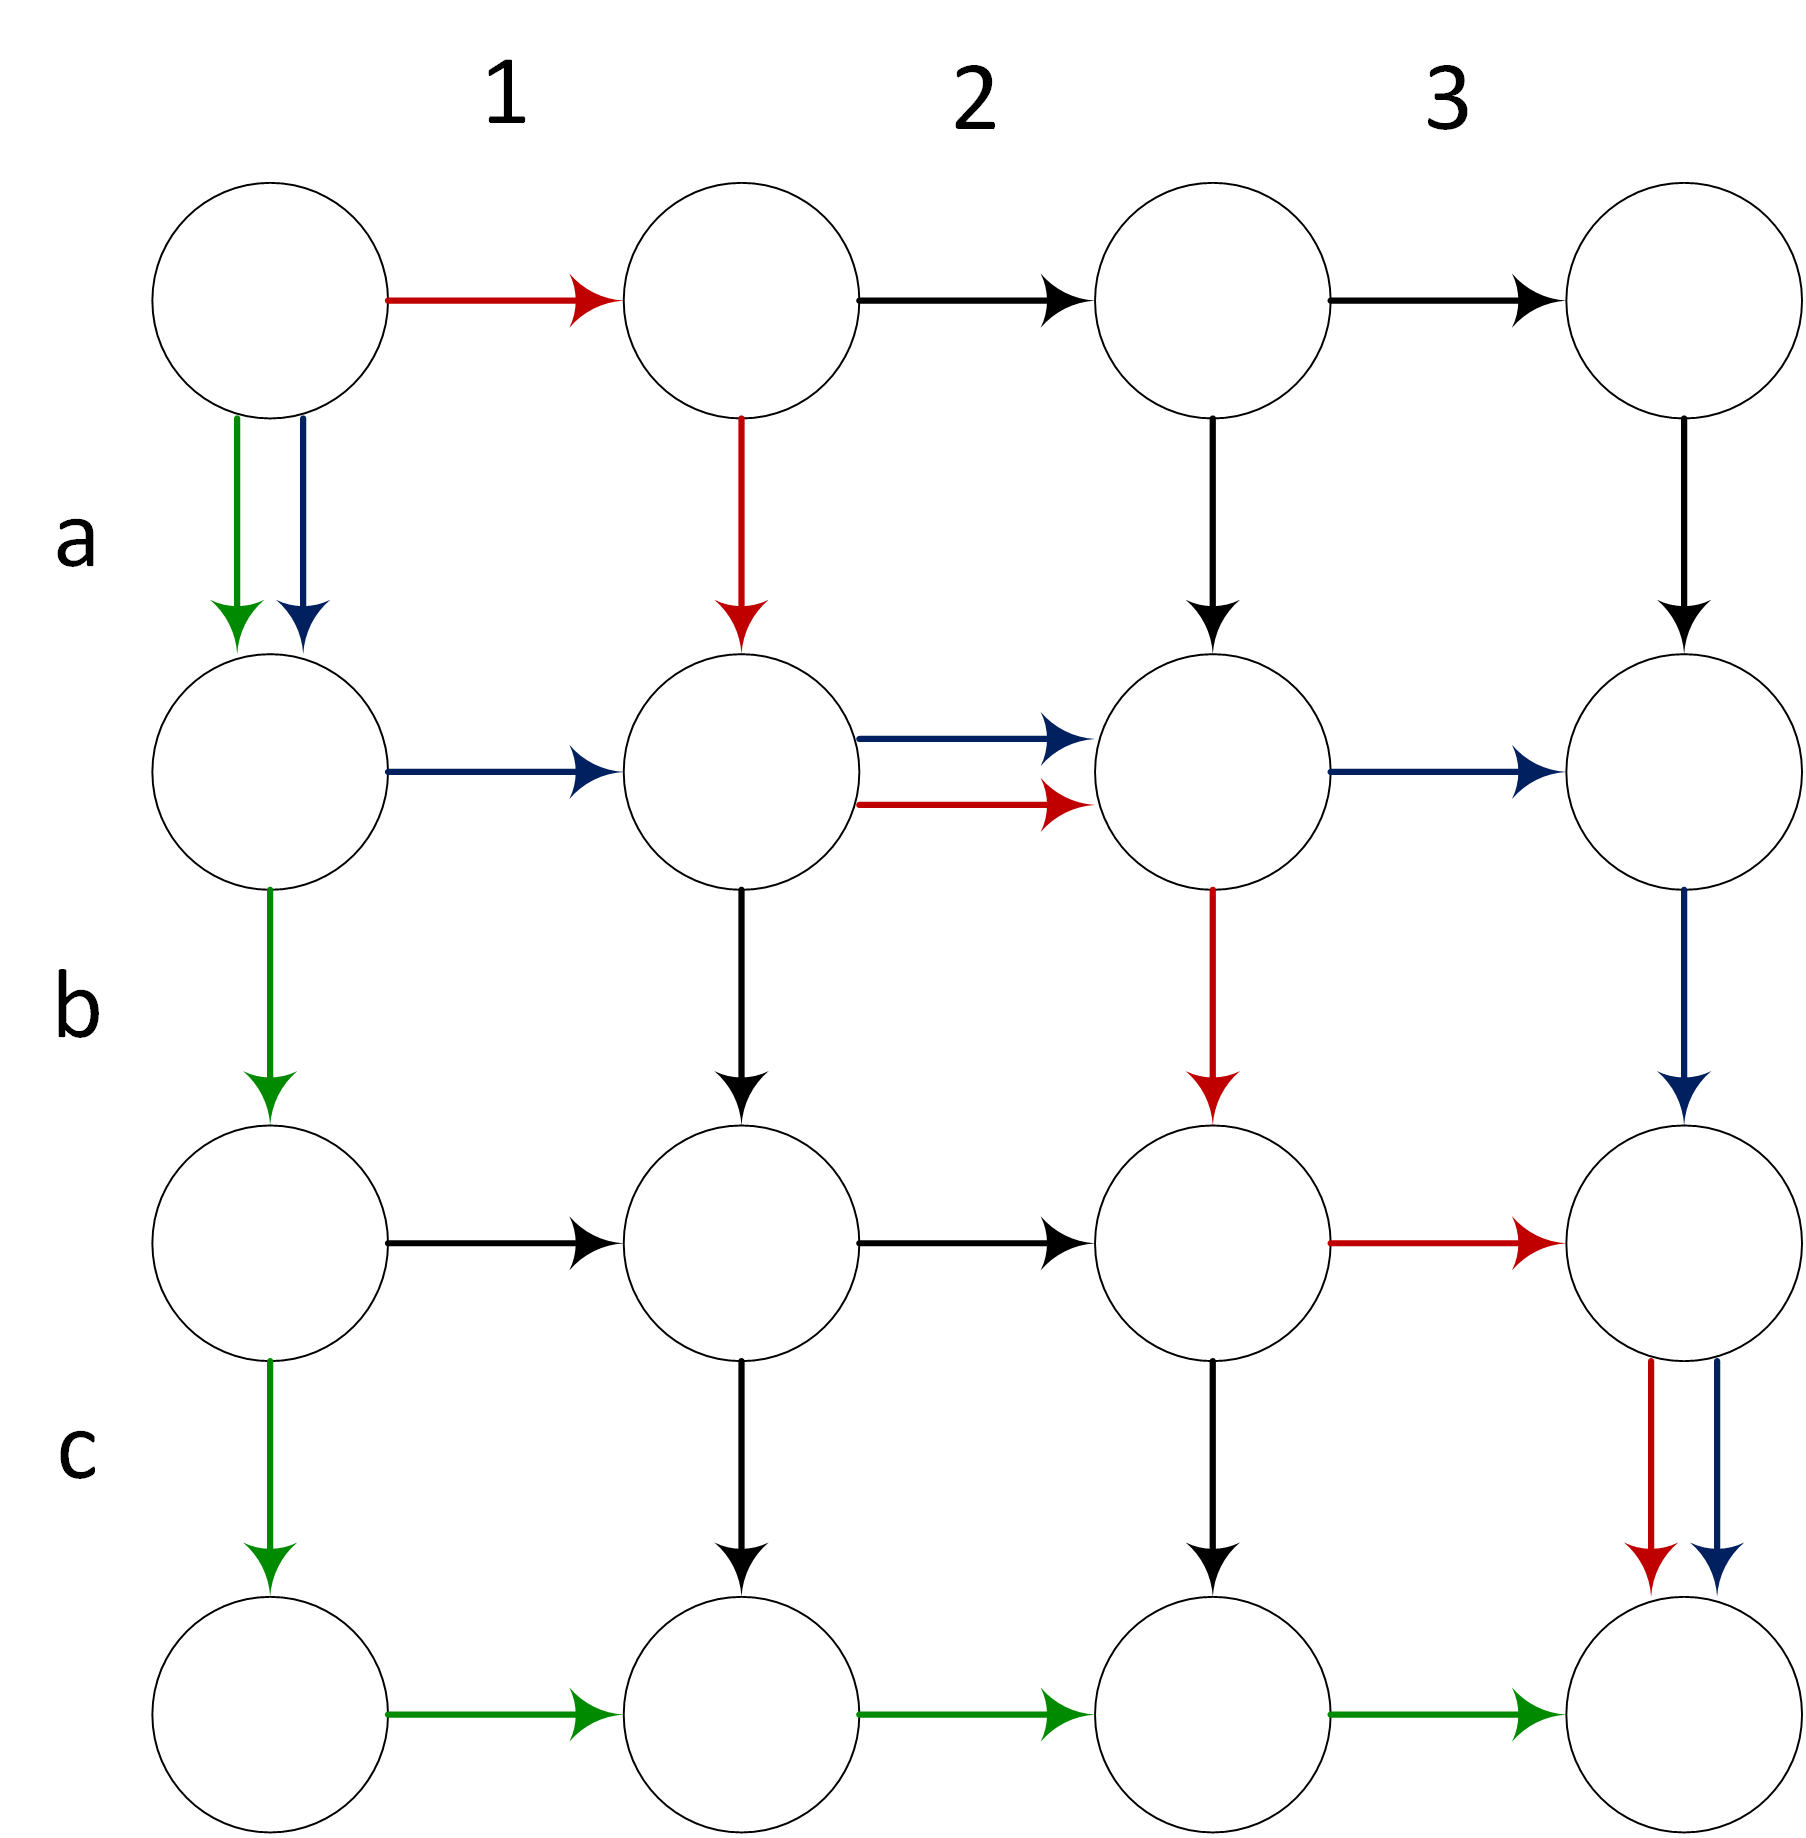
\includegraphics[width=.4\textwidth]{Nondeterminism}\\
\\
Da bei jedem Test der Zeitplaner eine andere Ausführungsreihenfolge (Umstände des Wettrennens, engl. race conditions) wählen kann, ist der Test praktisch nicht reproduzierbar. Wegen der großen Anzahl möglicher Abläufe ist ein systematisches Testen aussichtslos ("`Zustandsexplosion"').
Der Entwickler muss deshalb die Korrektheit seines Programms mathematisch beweisen (verifizieren). Um Flüchtigkeitsfehler und übersehene Spezialfälle auszuschließen, lässt man die Beweise maschinell überprüfen (formale Verifikation).
\\
Threads sind asynchron, d.h. sie laufen mit versch. Geschwindigkeiten. Es treten Wartezeiten auf, deren Zeitpunkt und Dauer nicht vorhersehbar ist, z.B. Laden einer neuen Speicherseite („page fault“), oder ein Zugriff auf den Zwischenspeicher (cache) scheitert.

\section{Kritische Bereiche}
Beispiel:\\
Zähler \texttt{z} wird initialisiert mit 0. Jeder Thread (von z.B. 10.000) addiert 1 zu \texttt{z}. \texttt{z++} wird vom Compiler sinngemäß so übersetzt:\\
\\
\texttt{1 \ int temp = z;} \\
\texttt{2 \ temp = temp + 1;} \\
\texttt{3 \ z = temp;} \\
\\
\texttt{z} ist eine gemeinsame Variable (gemeinsamer Speicher, shared memory), \texttt{temp} ist eine lokale Variable (temporäre Variable).
Jeder Thread hat seine eigene Version von \texttt{temp}.\\
\\
Beispielablauf für 3 Threads T1, T2, T3:
\begin{center}
\begin{tabular}{c|c|c|c|c|c|c}
\multicolumn{2}{c|}{\textbf{T1}} & \multicolumn{2}{c|}{\textbf{T2}} & \multicolumn{2}{c|}{\textbf{T3}} & \textbf{z} \\ \hline
\emph{Zeile} & \emph{temp1} & \emph{Zeile} & \emph{temp2} & \emph{Zeile} & \emph{temp3} & 0 \\ \cline{1-6}
1 & 0 & {} & {} & {} & {} & {} \\
{} & {} & 1 & 0 & {} & {} & {} \\ 
{} & {} & 2 & 1 & {} & {} & {} \\ 
{} & {} & 3 & {} & {} & {} & 1 \\ 
{} & {} & {} & {} & 1 & 1 & {} \\ 
{} & {} & {} & {} & 2 & 2 & {} \\ 
{} & {} & {} & {} & 3 & {} & 2 \\ 
2 & 1 & {} & {} & {} & {} & {} \\ 
3 & {} & {} & {} & {} & {} & 1 \\ 
\end{tabular}
\end{center}

Der Wert von \texttt{z} sollte am Ende 3 sein. T1, T2, T3 kommen sich gegenseitig in die Quere: Einmischung (interference). Einmischung kann es nur über gemeinsame Variablen geben.
Eine Methode, um Einmischung zu verhindern ist die Verwendung von \emph{kritischen Bereichen}.

\begin{description}
\item[Kritischer Bereich (auch kritischer Abschnitt, Emil. critical region, critical section)] Programmfragment in dem sich zu jedem Zeitpunkt höchstens ein Thread befindet.
\item[Gegenseitiger Ausschluss (mutual exclusion, exklusives Betriebsmittel)]
Wenn sich ein Thread in einem kritischen Bereich befindet, dann werden alle anderen Threads davon abgehalten, den kritischen Bereich zu betreten.
\end{description}

Beispiele für exklusive Betriebsmittel:
\begin{itemize}
\item Stuhl
\item Rechnerkern
\item Schreibzugriff auf Speicherblock
\item Schreibzugriff auf Bus
\item Drucker
\item Soundkarte (?)
\end{itemize}

Beispiel für einen kritischen Bereich:\\
\texttt{gemeinsam int z = 0; // Deklaration der gem. Var. z}\\
\texttt{kritisch z \{}\\
\texttt{z++ // kritischer Bereich, nur hier darf auf z zugegriffen werden}\\ % TODO: Einrücken
\texttt{\}}\\
\\
Wenn kritische Bereiche als Sprachmittel gegeben sind, kann der Compiler die korrekte Verwendung derselben überprüfen.\\
Der kritische Bereich kann von mehreren Threads nicht echt nebeneinander abgearbeitet werden, er wird also von den Threads in einer gewissen Reihenfolge nacheinander abgearbeitet (\emph{Serialisierbarkeit}). Zwischenzustände sind von anderen Threads nicht beobachtbar, weil die gemeinsamen Variablen nur im kritischen Bereich zugreifbar sind. Der kritische Bereich wirkt wie eine einzelne Aktion: er ist \emph{unteilbar} (atomar, engl. atomic).

\section{Sperren}
\begin{description}
\item[Sperre (lock)] Datenstruktur mit Operationen belegen und freigeben.
\item[erzeugen(l)] legt Sperre \texttt{l} an und initialisiert \texttt{l.frei} mit \texttt{false} (\texttt{l.frei}: Sperre frei).
\item[belegen(l)] wartet solange, bis \texttt{l.frei} den Wert \texttt{true} hat und setzt es dann auf \texttt{false}.
\item[freigeben(l)] Setzt \texttt{l.frei} auf \texttt{true}.
\end{description}

Sperren können verwendet werden, um kritische Bereiche zu implementieren.\\
Beispiel: Sperre \texttt{l} bewacht die gemeinsame Variable \texttt{z}.\\
Programm (HP):\\
\\
\texttt{Sperre l anlegen mit l.frei = false}\\
\texttt{Threads anlegen}
\texttt{Setze gem. Var. z = 0}\\
\texttt{freigeben(l)}\\

In jedem Thread:\\
\\
\texttt{0 \ belegen(l);} \\
\texttt{1 \ int temp = z;} \\
\texttt{2 \ temp = temp + 1;} \\
\texttt{3 \ z = temp;} \\
\texttt{4 \ freigeben(l);}
\\

Paradox: Um kritische Bereiche nutzen zu können, braucht man schon kritische Bereiche.

Beispielablauf für 2 Threads:
\begin{center}
\begin{tabular}{c|c|c|c|c|c|c}
\multicolumn{2}{c|}{\textbf{T1}} & \multicolumn{2}{c|}{\textbf{T2}} & \textbf{z} & \textbf{l.frei} & \textbf{Bemerkung} \\ \hline
\emph{Zeile} & \emph{temp1} & \emph{Zeile} & \emph{temp2} & 0 & true & {} \\ \cline{1-4}
0 & {} & {} & {} & {} & false & {} \\
{} & {} & 0 & {} & {} & {} & T2 wartet in Zeile 0 \\
1 & 0 & 0 & {} & {} & {} & {} \\
2 & 1 & 0 & {} & {} & {} & {} \\
3 & {} & 0 & {} & 1 & {} & {} \\
4 & {} & 0 & {} & {} & true & {} \\
{} & {} & 0 & {} & {} & false & Ende der Wartezeit \\
{} & {} & 1 & 1 & {} & {} & {} \\
{} & {} & 2 & 2 & {} & {} & {} \\
{} & {} & 3 & {} & 2 & {} & {} \\
{} & {} & 4 & {} & {} & true & {} \\
\end{tabular}
\end{center}

Sprechweise:
\begin{itemize}
\item Thread bewirbt sich für die Sperre (= ruft \texttt{belegen(l)} auf )
\item Thread besitzt Sperre \texttt{l} (= ist im krit. Bereich/hat \texttt{belegen(l)} erfolgreich aufgerufen)
\item Thread erwirbt die Sperre \texttt{l} (= betritt den krit. Bereich), Streit um die Sperre (engl. lock contention)
\end{itemize}